%
% fehlerfunktion.tex
%
% (c) 2021 Prof Dr Andreas Müller, OST Ostschweizer Fachhochschule
%
\section{Die Fehlerfunktion
\label{buch:integrale:section:fehlerfunktion}}
\rhead{Fehlerfunktion}
Die Wahrscheinlichkeitsdichte einer normalverteilten Zufallsvariable $X$
mit Erwartungswert $\mu$ und Varianz $\sigma^2$ ist
\begin{equation}
\varphi(x)
=
\frac{1}{\sqrt{2\pi}\sigma}
e^{-\frac{(x-\mu)^2}{2\sigma^2}}.
\label{buch:integrale:eqn:normaldichte}
\end{equation}
Die Verteilungsfunktion der Zufallsvariable ist dann durch das Integral
\begin{equation}
f(x)
=
F_X(x)
=
P(X\le x)
=
\frac{1}{\sqrt{2\pi}\sigma}
\int_{-\infty}^x 
e^{-\frac{(t-\mu)^2}{2\sigma^2}}
\,dt
\label{buch:integrale:eqn:normalverteilung}
\end{equation}
gegeben.
Die Erfahrung zeigt, dass es nicht möglich ist, das
Integral~\eqref{buch:integrale:eqn:normalverteilung}
in geschlossener Form auszuwerten.
Die Funktion $F_X(x)$ ist offenbar eine in Anwendungen nützliche und
häufig gebrauchte Funktion, die es verdient, in eine Standardbibliothek
von Funktion aufgenommen zu werden.
Dabei soll auch berücksichtigt werden, dass die neu zu definierende
spezielle Funktion möglichst auch für andere Anwendungen verwendet
werden kann, wie zum Beispiel die Berechnung gewisser Laplace-Transformierter.
Im Folgenden soll gezeigt werden, in welcher Form genau dies geschehen
kann.

%
% Vereinfachung des Integrals durch Standardisierung
%
\subsection{Standardisierung}
Die Formel~\ref{buch:integrale:eqn:normalverteilung} enthält die zwei 
Parameter $\mu$ und $\sigma$, sie ist daher als Basis für eine neue
spezielle Funktion nicht geeignet.
In diesem Abschnitt sollen sie eliminiert werden mit dem Ziel, ein
neues, einfacheres Integral zu definieren, aus dem sich 
\ref{buch:integrale:eqn:normalverteilung} leicht berechnen lässt.

\subsubsection{Elimination der Parameter $\mu$ und $\sigma$}
Aus der Wahrscheinlichkeitstheorie ist bekannt, dass zu einer
Zufallsvariablen $X$ mit Erwartungswert $E(X)=\mu$ und Varianz
$\operatorname{var}(X)=\sigma^2$ immer eine Zufallsvariable
gefunden werden kann mit Erwartungswert $0$ und Varianz $1$.
Tatsächlich bekommt man für die standardisierte Zufallsvariable
\begin{equation}
Z = \frac{X-\mu}{\sigma}
\label{buch:integrale:eqn:standardisierung}
\end{equation}
die Werte
\begin{align*}
E(Z)
&=
E\biggl(\frac{X-\mu}{\sigma}\biggr)
=
\frac{E(X)-\mu}{\sigma}
=
\frac{\mu-\mu}{\sigma}
=
0
\\
\text{und}\qquad
\operatorname{var}(Z)
&=
\operatorname{var}\biggl(\frac{X-\mu}{\sigma}\biggr)
=
\frac{\operatorname{var}(X)}{\sigma^2}
=
1,
\end{align*}
wie versprochen.
Dies bedeutet, dass sich das Integral~\ref{buch:integrale:eqn:normalverteilung}
durch ein Integral ausdrücken lassen muss, in der die Parameter $\mu$
und $\sigma$ nicht mehr vorkommen.

Die Standardisierungsformel~\eqref{buch:integrale:eqn:standardisierung}
deutet auch bereits an, wie man das
Integral~\ref{buch:integrale:eqn:normalverteilung} vereinfachen kann.
Dazu führen wir die Substitution $z=(t-\mu)/\sigma$ aus und erhalten
\begin{align*}
f(x)
&=
\frac{1}{\sqrt{2\pi}\sigma} 
\int_{-\infty}^x e^{-\frac{(t-\mu)^2}{2\sigma^2}}\,dt
=
\frac{1}{\sqrt{2\pi}\sigma}
\int_{\infty}^{(x-\mu)/\sigma}
e^{-\frac{z^2}2}\,\sigma dz
=
\frac{1}{\sqrt{2\pi}}
\int_{-\infty}^{\frac{x-\mu}{\sigma}} e^{-\frac{z^2}2}\,dz.
\end{align*}
Das Integral auf der rechten Seite enthält die Parameter $\mu$ und
$\sigma$ nur noch in der Integrationsgrenze.
Es kann durch die Wahrscheinlichkeitsverteilungsfunktion der
Standardnormalverteilung
\begin{equation}
\Phi(x) = \frac{1}{\sqrt{2\pi}} \int_{-\infty}^x e^{-\frac{z^2}2}\,dz
\label{buch:integrale:eqn:standardnormalverteilung}
\end{equation}
ausgedrückt werden, es ist
\[
F_X(x) = \Phi\biggl(\frac{x-\mu}{\sigma}\biggr).
\]
Die Funktion $\Phi(x)$ ist daher in guter Kandidate für eine neue spezielle
Funktion.

\subsubsection{Die Funktion $\operatorname{erf}(x)$}
Die Funktion \eqref{buch:integrale:eqn:standardnormalverteilung} hat
einige Nachteile, die sich als Barriere für die numerische 
Berechnung der Funktionswerte herausstellen könnte.

Zunächst ist $\Phi(x)$ als ein uneigentliches Integral definiert.
Eine direkte numerische Integration muss daher über ein sehr grosses
Interval erstreckt werden, um die Genauigkeit garantieren zu können.
Jedoch ist bekannt, dass $\Phi(0)=\frac12$, denn
\[
\Phi(0)
=
\frac{1}{\sqrt{2\pi}}
\int_{-\infty}^0 e^{-\frac{z^2}2}\,dz
=
\frac12\cdot\underbrace{\frac{1}{\sqrt{2\pi}}
\int_{-\infty}^{\infty} e^{-\frac{z^2}2}\,dz}_{\displaystyle=1}
=
\frac12.
\]
Man kann daher schreiben
\begin{equation}
\Phi(x) = \frac12 + \frac{1}{\sqrt{2\pi}}\int_0^x e^{-\frac{z^2}{z}}\,dz.
\label{buch:integrale:eqn:Phireduziert}
\end{equation}
Das Integral auf der rechten Seite ist ein gewöhnliches Integral und ist
damit viel einfacher zu berechnen.

Am Integral in~\eqref{buch:integrale:eqn:Phireduziert} ist aber noch etwas
unerfreulich, dass der Exponent komplizierter ist als nötig.
Mit Hilfe der Variablentransformation $u = z/\sqrt{2}$ erhalten wir
aus dem Integral in~\eqref{buch:integrale:eqn:Phireduziert}
\begin{align*}
\frac{1}{\sqrt{2\pi}}
\int_0^x e^{-\frac{z^2}2}\,dz
=
\frac{1}{\sqrt{2\pi}}
\int_0^{x/\sqrt{2}}
e^{-u^2} \, \sqrt{2}\,du
=
\frac{1}{\sqrt{\pi}}
\int_0^{x/\sqrt{2}}
e^{-u^2} \,du.
\end{align*}
Damit sind wir bei einer Funktion angekommen, die sich gut als spezielle
Funktion eignet.

\begin{definition}
Die Fehlerfunktion $\operatorname{erf}(x)$ ist die Funktion
\index{Fehlerfunktion}%
\index{erf(x)@$\operatorname{erf}(x)$}%
\[
\operatorname{erf}
\colon
\mathbb{R}\to [-1,1]
:
x
\mapsto
\operatorname{erf}(x)
:=
\frac{2}{\pi}
\int_0^x e^{-u^2}\,du.
\]
\end{definition}

\begin{figure}
\centering
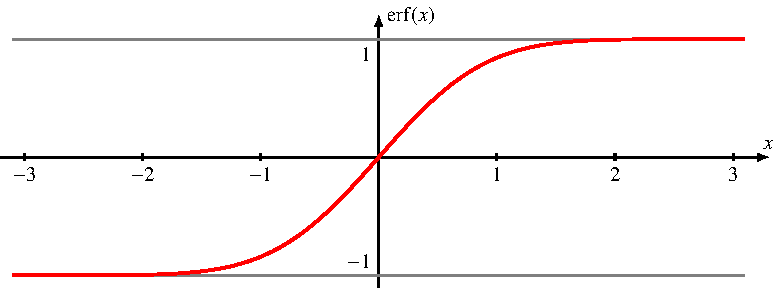
\includegraphics{chapters/060-integral/images/erf.pdf}
\caption{Graph der Fehlerfunktion $\operatorname{erf}(x)$
\label{buch:integrale:fig:erf}}
\end{figure}
Die Funktion $\operatorname{erf}$ nimmt Werte zwischen $-1$ und $1$ an,
wie man in Abbildung~\ref{buch:integrale:fig:erf} sehen kann.
Die horizontalen Geraden $y=\pm 1$ sind Asymptoten.
Die exakte Berechnung von $\operatorname{erf}(x)$ für sehr grosse Werte
des Argumentes gestaltet sich schwierig, da es zur starker Auslöschung
kommen kann.
Da die Funktionswerte $\operatorname{erf}(x)$ sehr nahe bei $1$ sind,
lohnt es sich, nicht $\operatorname{erf}(x)$, sondern $1-\operatorname{erf}(x)$
zu berechnen.

\begin{definition}
\index{komplementäre Fehlerfunktion}
\index{Fehlerfunktion, komplementäre}
\index{erfc(x)@$\operatorname{erfc}(x)$}
Die {\em komplementäre Fehlerfunktion} ist die Funktion
\[
\operatorname{erfc}
\colon
\mathbb{R} \to [0,2]
:
x\mapsto
\operatorname{erfc}(x)
:=
1-\operatorname{erf}(x)
=
\frac{2}{\sqrt{\pi}}\int_x^\infty e^{-u^2}\,du.
\]
Die {\em verallgemeinerte Fehlerfunktion} ist definiert als
\[
\operatorname{erf}(a,b)
=
\frac{2}{\sqrt{\pi}}
\int_a^b e^{-u^2}\,du.
\]
\end{definition}

Mit der Fehlerfunktion kann die Standardnormalverteilungsfunktion jetzt
als
\[
\Phi(x)
=
\frac12
+
\frac12\operatorname{erf}\biggl( \frac{x}{\sqrt{2}} \biggr)
=
\frac12\biggl(
1+\operatorname{erf}\biggl(\frac{x}{\sqrt{2}}\biggr)\biggr)
\]
ausdrücken.
Die Verteilungsfunktion einer normalverteilten Zufallsvariable mit
Erwartungswert $\mu$ und Varianz $\sigma^2$ kann ebenfalls mit
\[
F_X(x)
=
\frac12\biggl(
1+\operatorname{erf}\biggl(\frac{x-\mu}{\sqrt{2}\sigma}\biggr)
\biggr)
\]
berechnet werden.
Die Fehlerfunktion ist also eine ``gute'' spezielle Funktion, die
die Berechnung von Wahrscheinlichkeitswerten von normalverteilten
Zufallsvariablen vereinfacht.

\subsubsection{Fehlerfunktion als hypergeometrische Funktion}
Die Fehlerfunktion ist eine Stammfunktion von
\[
\frac{2}{\sqrt{\pi}}
e^{-x^2}
=
\frac{2}{\sqrt{\pi}}
\biggl(
1 - \frac{x^2}{1!} + \frac{x^4}{2!} - \frac{x^6}{3!} + \frac{x^8}{4!}-\dots
\biggr).
\]
Durch gliedweises Integrieren erhaält man
\begin{align*}
\operatorname{erf}(x)
&=
\frac{2}{\sqrt{\pi}}
\biggl(
x - \frac{x^3}{1!\cdot 3} + \frac{x^5}{2!\cdot 5} - \frac{x^7}{3!\cdot 7} + \frac{x^9}{4!\cdot 9}-\dots
\biggr)
\intertext{Ein gemeinsamer Faktor $x$ kann ausgeklammert werden.
Die alternierenden Vorzeichen und die in Zweierschritten ansteigenden
Potenzen bedeuten, dass der Klammerausdruck als Reihe}
&=
\frac{2x}{\sqrt{\pi}}
\biggl(
1 +
\frac13\cdot\frac{(-x^2)^1}{1!}
+
\frac15\cdot\frac{(-x^2)^2}{2!}
+
\frac17\cdot\frac{(-x^2)^3}{3!}
+
\frac19\cdot\frac{(-x^2)^4}{4!}
+
\dots
+
\frac{1}{2k+1}\frac{(-x^2)^k}{k!}
+
\dots
\biggr)
\intertext{in $-x^2$ geschrieben werden kann.
Der Koeffzient $1/(2k+1)$ muss jetzt noch mit Pochhammer-Symbolen 
geschrieben werden.
Dazu wird er zunächst als $\frac12\cdot 1/(k+\frac12)$ geschrieben,
weil der Nenner dann in Einerschritten anwächst, wie dies für
Pochhammer-Symbole benötigt wird.
Das Pochhammer-Symbol $(\frac32)_k$ hat den korrekten letzten Faktor
$k+\frac12$, aber es hat viele zusätzliche Faktoren, nämlich
alle Faktoren in $(\frac12)_k$ ausser dem ersten.
Mit einem geeigneten Zähler können diese wieder zum Verschwinden
gebracht werden.
So erhält man die Darstellung
}
&=
\frac{2x}{\sqrt{\pi}}
\sum_{k=0}^\infty
\frac{1}{2\cdot (k+\frac12)}
\frac{(-x^2)^k}{k!}
=
\frac{2x}{\sqrt{\pi}}
\sum_{k=0}^\infty
\frac{1}{2} \cdot\frac{1}{k+\frac12}
\frac{(-x^2)^k}{k!}
\\
&=
\frac{2x}{\sqrt{\pi}}
\sum_{k=0}^\infty
\frac12
\cdot
\frac{
\frac32
\cdot \frac52
\cdot\ldots\cdot(k-\frac12)
\phantom{\mathstrut\cdot(k+\frac12)}
}{
\frac32
\cdot \frac52
\cdot\ldots\cdot(k-\frac12)\cdot(k+\frac12)
}
\frac{(-x^2)^k}{k!}
\\
&=
\frac{2x}{\sqrt{\pi}}
\sum_{k=0}^\infty
\frac{
\frac12
\cdot
\frac32
\cdot \frac52
\cdot\ldots\cdot(k-\frac12)
\phantom{\mathstrut\cdot(k+\frac12)}
}{
\phantom{\frac12\cdot\mathstrut}
\frac32
\cdot \frac52
\cdot\ldots\cdot(k-\frac12)\cdot(k+\frac12)
}
\frac{(-x^2)^k}{k!}
\\
&=
\frac{2x}{\sqrt{\pi}}
\sum_{k=0}^\infty \frac{(\frac12)_k}{(\frac32)_k}\frac{(-x^2)^k}{k!}
=
\frac{2x}{\sqrt{\pi}}
\,
\mathstrut_1F_1\biggl(
\begin{matrix}\frac12\\\frac32\end{matrix}; -x^2
\biggr)
\end{align*}
der Fehlerfunktion als hypergeometrische Funktion.

%
% Laplace-Transformation der Fehlerfunktion
%
\subsection{Laplace-Transformation}
Wir berechnen die Laplace-Transformierte der Funktion
\[
f(t) = \operatorname{erf}\biggl(\frac{a}{2\sqrt{t}}\biggr).
\]
Nach Definition der Laplace-Transformation ist dies die Funktion
\begin{align*}
\mathscr{L}f(s)
&=
\int_0^\infty
e^{-st} \operatorname{erf}\biggl(\frac{a}{2\sqrt{t}}\biggr)
\,dt
=
\int_0^\infty
e^{-st}
\frac{2}{\sqrt{\pi}}
\int_0^{\frac{a}{2\sqrt{t}}}
e^{-x^2}
\,dx
\,dt.
\end{align*}
Das Integrationsgebiet $G$ ist der Teil des ersten Quadranten der
$t$-$x$-Ebene, für den die Ungleichung $x \le a/2\sqrt{t}$ gilt.
Dies ist gleichbedeutend mit $t \le a^2/4x^2$.
Vertauscht man die Integrationsreihenfolge, erhält man
\begin{align}
\mathscr{L}f(s)
&=
\int_G
e^{-st}
\frac{2}{\sqrt{\pi}}
e^{-x^2}
\,dx \,dt
=
\int_0^\infty
\int_0^{\frac{a^2}{4x^2}}
e^{-st}
\frac{2}{\sqrt{\pi}}
e^{-x^2}
\,dt
\,dx
=
\frac{2}{\sqrt{\pi}}
\int_0^\infty
e^{-x^2}
\int_0^{\frac{a^2}{4x^2}}
e^{-st}
\,dt
\,dx
\notag
\\
&=
\frac{2}{\sqrt{\pi}}
\int_0^\infty
e^{-x^2}
\biggl[
-\frac1{s}e^{-st}
\biggr]_0^{\frac{a^2}{4x^2}}
\,dx
=
\frac{2}{\sqrt{\pi}}
\int_0^\infty
e^{-x^2}
\frac1{s}
\biggl(
1-e^{-\frac{sa^2}{4x^2}}
\biggr)
\,dx
\notag
\\
&=
\frac{1}{s}
\cdot
\frac{2}{\sqrt{\pi}}\int_0^\infty e^{-x^2}\,dx
-
\frac1{s}
\cdot
\frac{2}{\sqrt{\pi}}
\int_0^\infty
e^{-x^2-\frac{sa^2}{4x^2}}
\,dx
\notag
\\
&=
\frac1s\lim_{x\to\infty} \operatorname{erf}(x)
-
\frac1s
\cdot
\frac{2}{\sqrt{\pi}}
\int_0^\infty e^{-\left(x^2+\frac{sa^2}{4x^2}\right)}\,dx.
\label{buch:integrale:eqn:laplaceerf}
\end{align}
Der Grenzwert im ersten Term ist $1$, nach Definition der Fehlerfunktion. 
Schreiben wir $b=a\sqrt{s}/2$, dann wird das Integral im zweiten Term
\begin{equation}
I(b)
=
\int_0^\infty e^{-\left(x^2+\frac{sa^2}{4x^2}\right)}\,dx
=
\int_0^\infty \exp\biggl(-\biggl(x^2+\frac{b^2}{x^2}\biggr)\biggr)\,dx.
\label{buch:integrale:eqn:Ibsumme}
\end{equation}
Den Exponenten im Integranden kann man wie folgt als quadratischen
Ausdruck in $x\pm a/x$ schreiben:
\begin{equation*}
\begin{aligned}
%\biggl(
x^2 + \frac{b^2}{x^2}
%\biggr)
&=
\biggl(x+\frac{b}{x}\biggr)^2 - 2b
\\
&=
\biggl(x-\frac{b}{x}\biggr)^2 + 2b.
\end{aligned}
\end{equation*}
Man kann also das Integral $I(b)$ auf die eine oder andere Art als
\begin{equation}
\begin{aligned}
I(b)
&=
\int_0^\infty \exp\biggl(-\biggl(x+\frac{b}{x}\biggr)^2+2b\biggr)\,dx
\\
\text{oder}\quad\phantom{I(b)}
&=
\int_0^\infty \exp\biggl(-\biggl(x-\frac{b}{x}\biggr)^2-2b\biggr)\,dx
\end{aligned}
\label{buch:integrale:eqn:fehlerintegrale}
\end{equation}
schreiben.
Die Faktoren $e^{\pm 2b}$ können aus dem Integral genommen werden.
Trotzdem kann man das Integral nicht einfach ausführen.

Die Substitution $y=x\pm\frac{b}{x}$ vereinfacht den Integranden
\eqref{buch:integrale:eqn:fehlerintegrale}
zwar zu $e^{-y^2}$, aber die Substitution für $dx$ liefert
\begin{equation}
y=x\pm\frac{b}{x}
\qquad\Rightarrow\qquad
dy = \biggl(1\mp \frac{b}{x^2}\biggr)\,dx.
\label{buch:integrale:eqn:dy}
\end{equation}
Dies kann für die Berechnung von $I(b)$ verwendet werden.
Zunächst folgt aus \eqref{buch:integrale:eqn:fehlerintegrale},
dass jede konvexe Kombination der beiden Integrale mit Koeffizienten,
die sich zu $1$ summieren, wieder $I(b)$ erbibt.
Wählen wir die Koeffizienten 
\[
\frac12\biggl(1\mp\frac{b}{x^2}\biggr),
\]
dann heben sich die Terme mit $b/x^2$ weg, wir erhalten die
konvexe Kombination
\[
I(b)
=
\frac12
\cdot
\underbrace{
\int_0^\infty
\biggl(1-\frac{b}{x^2}\biggr)
\exp\biggl(-\biggl(x+\frac{b}{x}\biggr)^2\biggr)\,dx
}_{\displaystyle=I_+(b)}
\mathstrut
\cdot e^{2b}
+
\frac12
\underbrace{
\int_0^\infty
\biggl(1+\frac{b}{x^2}\biggr)
\exp\biggl(-\biggl(x-\frac{b}{x}\biggr)^2\biggr)\,dx
}_{\displaystyle=I_-(b)}
\mathstrut
\cdot e^{-2b},
\]
die aus zwei Integralen besteht, die einfacher berechnet werden können.

Im Integral $I_-(b)$ können wir die Substition \eqref{buch:integrale:eqn:dy}
und erhalten
\begin{align*}
I_-(b)
&=
\int_{-\infty}^\infty
\biggl(1+\frac{b}{x^2}\biggr)
\exp\biggl(-\biggl(x-\frac{b}{x}\biggr)^2\biggr)\,dx
=
\int_{-\infty}^\infty e^{-y^2}\,dy
=
\frac{\sqrt{\pi}}2
\end{align*}
nach Definition der Fehlerfunktion.

Das erste Integral $I_+(b)$ ist etwas schwieriger zu berechnen.
Die Substition $z=b/x$ bildet das Integrationsinterval auf sich selbst ab,
aber die Integrationsrichtung kehrt um.
Mit
\[
dz = -\frac{b}{x^2}\,dx
\qquad\Rightarrow\qquad
dx = -\frac{z^2}{b}\,dz
\]
erhalten wir jetzt
\begin{align*}
I_+(b)
&=
\int_0^\infty
\biggl(1-\frac{b}{x^2}\biggr)
\exp\biggl(-\biggl(x+\frac{b}{x}\biggr)^2\biggr)\,dx
\\
&=
\int_{\infty}^0
\biggl(1-\frac{b}{b^2/z^2}\biggr)
\exp\biggl(-\biggl(\frac{b}{z}+z\biggr)^2\biggr)\,
\biggl(-\frac{b}{z^2}\biggr)\,dz
\\
&=
\int_{0}^{\infty}
\biggl(1-\frac{b}{b^2/z^2}\biggr)
\exp\biggl(-\biggl(\frac{b}{z}+z\biggr)^2\biggr)\,
\frac{b}{z^2}\,dz
\\
&=
\int_{0}^{\infty}
\biggl(\frac{b}{z^2}-1\biggr)
\exp\biggl(-\biggl(\frac{b}{z}+z\biggr)^2\biggr)\,
dz
=
-I_+(b).
\end{align*}
Indem man auf beiden Seiten $I_+(b)$ addiert erhält man nun $2I_+(b)=0$,
also auch $I_+(b)=0$.
Das Integral $I_+(b)$ verschwindet also, $I_+(b)=0$.

Nach all diesen Zwischenrechnungen können wir jetzt das Integral $I(b)$
zusammensetzen.
Wir finden
\begin{align*}
I(b)
&=
\frac12e^{2b} I_+(b) +\frac12e^{-2b} I_-(b)
\\
&=
\frac12e^{-a\sqrt{s}}\cdot \frac{\sqrt{\pi}}{2}.
\end{align*}
Einsetzen in \eqref{buch:integrale:eqn:laplaceerf} gibt jetzt das
Resultat für die Laplace-Transformierte von $f(t)$, sie ist
\[
\mathscr{L}f(s)
=
\frac1s - \frac1s\cdot\frac{2}{\sqrt{\pi}} I(b)
=
\frac1s\biggl(1-\frac12e^{-a\sqrt{s}} \biggr).
\]

\begin{satz}
\index{Satz!Laplace-Transformierte der Fehlerfunktion}%
Die Laplace-Transformierte der Fehlerfunktion mit Argument
$a/2\sqrt{t}$ ist
\begin{equation}
f(t) = \operatorname{erf}\biggl(\frac{a}{2\sqrt{t}}\biggr)
\qquad\multimapdotbothA\qquad
\mathscr{L}f(s)
=
\frac1s\biggl(1-\frac12e^{-a\sqrt{s}}\biggr).
\end{equation}
\end{satz}




\subsection{Berechnungsmethoden}
Die Fehlerfunktion kann natürlich mit numerischen Integrationsmethoden
berechnet werden.
Diese verlangen jedoch typischerweise die Auswertung des Integranden
an einer grossen Zahl von Stützstellen.
Im vorliegenden Falle müsste die transzendente Exponentialfunktion
sehr häufig berechnet werden, was zu sehr langer Laufzeit führt.
Gefragt sind daher Berechnungsverfahren, die möglichst nur arithmetische
Operationen verwenden, die sehr schnell in Hardware ausgeführt werden
können.

\subsubsection{Taylorreihe}
Die Fehlerfunktion ist das Integral einer Exponentialfunktion, die mit
Hilfe einer Potenzreihe für beliebige Argumente berechnet werden kann.
Aus
\[
e^x
=
1+x+\frac{x^2}{2!}+\frac{x^3}{3!} + \dots
=
\sum_{k=0}^\infty \frac{x^k}{k!}
\]
erhalten wir die Potenzreihe
\begin{equation}
e^{-t^2}
=
\sum_{k=0}^{\infty}
(-1)^k
\frac{t^{2k}}{k!},
\label{buch:integrale:eqn:erftaylor}
\end{equation}
die für alle Werte von $t$ konvergiert.

Da die Reihe
\eqref{buch:integrale:eqn:erftaylor}
absolut konvergiert, darf man sie gliedweise integrieren und erhält
\begin{equation}
\operatorname{erf}(x)
=
\frac{2}{\sqrt{\pi}}
\int_0^x
e^{-t^2}\,dt
=
\frac{2}{\sqrt{\pi}}
\sum_{k=0}^\infty \frac{(-1)^k}{k!}\int_0^x t^{2k}\,dt
=
\frac{2}{\sqrt{\pi}}
\sum_{k=0}^\infty \frac{(-1)^kx^{2k+1}}{k!(2k+1)}.
\label{buch:integrale:eqn:erfreihe}
\end{equation}
Diese Reihenentwicklung ist sehr effizient für kleine Werte von $x$.
Für grosse Werte von $x$ entstehen aber sehr grosse Zwischenterme in der
Reihe, was zu Auslöschung und damit zu Genauigkeitsverlust führt.

\subsubsection{Hypergeometrische Funktion}
Die Taylor-Reihe~\eqref{buch:integrale:eqn:erfreihe} der Fehlerfunktion
kann auch mit Hilfe hypergeometrischer Funktionen geschrieben werden.
Da nur ungerade Potenzen vorkommen, klammern wir zunächst einen gemeinsamen
Faktor $x$ aus:
\[
\operatorname{erf}(x)
=
\frac{2x}{\sqrt{\pi}}
\sum_{k=0}^\infty
\frac{1}{2k+1}
\frac{(-x^2)^k}{k!}.
\]
Der Bruch $1/(2k+1)$  muss jetzt noch mit Hilfe von Pochhammer-Symbolen
geschrieben werden.
Dazu beachten wir, dass
\begin{align*}
\frac{1}{2k+1} 
&=
\frac12
\frac{1}{\frac32+k-1}
\\
&=
\frac12
\frac{
\frac32(\frac32+1)(\frac32+2)\dots(\frac32+k-2)\phantom{(\frac32+k-1)}
}{
\frac32(\frac32+1)(\frac32+2)\dots(\frac32+k-2)(\frac32+k-1)
}
\\
&=
\frac{
\frac12(\frac12+1)(\frac12+2)(\frac12+3)\dots(\frac12+k-1)
}{
\frac32(\frac32+1)(\frac32+2)\dots(\frac32+k-2)(\frac32+k-1)
}
\\
&=
\frac{(\frac12)_k}{(\frac32)_k}.
\end{align*}
Somit ist die Fehlerfunktion als hypergeometrische Funktion
\[
\operatorname{erf}(x)
=
\frac{2x}{\sqrt{\pi}}\sum_{k=0}^\infty
\frac{(\frac12)_k}{(\frac32)_k}\frac{(-x^2)^k}{k!}
=
\frac{2x}{\sqrt{\pi}}\,
\mathstrut_1F_1({\textstyle\frac12};{\textstyle\frac32};-x^2).
\]
gegeben.

\subsubsection{Kettenbruchentwicklung}
Besonders für grosse $x$ interessiert man sich mehr für
$\operatorname{erfc}(x)$ als für $\operatorname{erf}(x)$.
Die Potenzreihe \eqref{buch:integrale:eqn:erfreihe} ist
dafür wegen der bereits erwähnten Auslöschung besonders ungeeignet.
Man kann aber die Kettenbruchentwicklung 
\begin{equation}
\operatorname{erfc}(z)
=
\frac{2ze^{-z^2}}{\sqrt{\pi}}
\cfrac{1}{
z+\cfrac{\frac12}{
z+\cfrac{\frac22}{
z+\cfrac{\frac32}{
z+\cfrac{\frac42}{
z+\cfrac{\frac52}{
z+\cfrac{\frac62}{
z+\dots}}}}}}}
\end{equation}
finden, die in \cite[p.~175]{buch:pade} dargestellt wird.
Für grosse $z$ liefert dieser Kettenbruch besonders schnell konvergierende
Näherungsbrüche für $\operatorname{erfc}(z)$.

\subsubsection{Interpolation}
Die GNU Scientific Library \cite{buch:library:gsl} verwendet eine Reihe von
Tschebyscheff-Approximationspolynomen, die für die Intervalle, in denen
sie definiert sind, besonders effizient zu berechnende Approximation
mit Maschinengenauigkeit ergeben.
